Research on various aspects of hovercraft design, mechanics and physics first principles, as well as input from the TA and the design decisions of peers, all influenced the current hovercraft designs. This document first describes the information discovered about the mechanics of a hovercraft, then proceeds by describing the designs, and summarizing the final product.

\subsection{Hovercraft Mechanics}
A hovercraft is able to move freely due to the minimum amount of friction between the vehicle and the ground. The chamber of air between the craft and ground, called the plenum chamber\footnote{http://en.wikipedia.org/wiki/Hovercraft}, is formed by the body of the hovercraft and a skirt. The air flowing into the plenum chamber forms a ring which keeps the external lower pressure out, ensuring the persistence of the internal air cushion. The amount of air entering the plenum chamber must be at least be equal to the amount of air that escapes underneath the skirt in order to keep the craft afloat. Further, it is incorrect to assume that air will escape evenly around the skirt’s perimeter. As more air is blown into the plenum chamber, the pressure of the air on the inside becomes higher than that on the outside, creating an upward force that lifts the hovercraft. When this upward pressure exactly matches the downward force of gravity, the desired floating effect is achieved. \cite{CambridgeJournals:370274} \cite{831309}

\subsubsection{Steering}
Different approaches have been taken to steer the craft. Larger hovercrafts typically employ a large propeller at the rear to drive the vehicle forward. Rudders\footnote{http://en.wikipedia.org/wiki/Rudder} are used for steering. Another option, usually seen in smaller hovercrafts, is to tilt the base, affecting the plenum chamber underneath. This results in a change in direction because a drag is created on one side, creating a pivot point.

 \begin{minipage}{6.5in}
  \begin{center}
    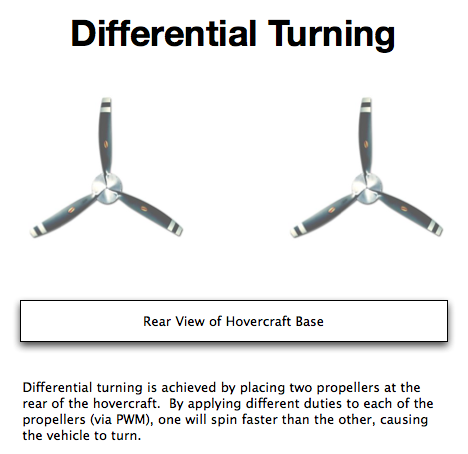
\includegraphics[width=85mm]{imageSources/differentialTurning.png}
  \end{center}
  \captionof{figure}{Differential Turning} 
  \label{differentialTurning}
  \end{minipage}

Instead of using 2 fans on the craft (one for filling the plenum chamber and one for forward thrust), a single propeller may be used for both functions. A fraction of the air intake is directed into the inner chamber to lift the craft, while the remaining air flow is forced behind the craft, creating thrust.

  \begin{minipage}{6.5in}
  \begin{center}
    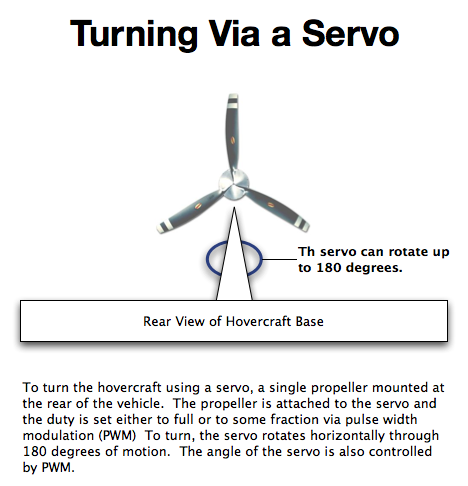
\includegraphics[width=85mm]{imageSources/servoTurning.png}
  \end{center}
  \captionof{figure}{Servo Turning} 
  \label{servoTurning}
  \end{minipage}

Steering may further be affected by either differential turning (Figure \ref{diffrentialTurning}) or though the use of a servo motor (Figure \ref{servoTurning}). The former approach commonly employs two thrust sources on either side of the vehicle. By altering the thrust of either motor (for example with pulse width modulation), one motor will be more powerful than the other, causing the craft to turn. The latter approach sees a propeller mounted to a servo motor. As the servo rotates through its 180 degree range, the thrust of the propeller is directed in a specific direction, also causing the craft to turn.

\subsubsection{Skirt}
An advancement in the development of the skirt is known as the Double-Walled Flexible Skirt, or more commonly the “Big Skirt”\footnote{http://www.freepatentsonline.com/3268021.html}. The design came about in the 1960’s by McReary. The idea was to inflate the outer skirt to allow the craft to move more freely over rough terrain and choppy water.

In general, the purpose of the skirt is to increase the overall surface area of the vehicle. By spreading the weight of the craft over a lager area, the pressure required to counteract this downward pressure is reduced. A common analogy is that of stepping on a single nail as opposed to lying on a bed of nails. Applying one’s entire weight on the small surface area of a single nail will surely result in a painful experience. However, by spreading one’s weight over the combined surface area of many nails, the pressure on any single point is reduced to the point where any particular nail cannot cause harm.

\subsection{Ground Effect}
Ground effect refers to the collection of aerodynamic effects felt by aircraft when flying in close proximity to the ground \footnote{http://www.google.ca/patents?hl=en\&lr=\&vid=USPAT4290500\&id=1iwBAAAAEBAJ\&oi=fnd\&dq=ground+effect+hovercraft}. If the hovercraft has too much lift, it is likely that it may well feel the effects of such a phenomenon.  An illustration of ground effect can be seen in Figure \ref{groundEffect}

  \begin{minipage}{6.5in}
  \begin{center}
    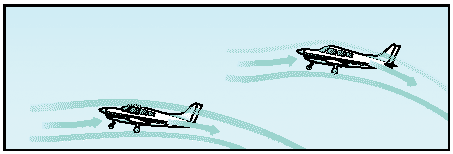
\includegraphics[width=85mm]{imageSources/groundEffect.png}
  \end{center}
  \captionof{figure}{Ground Effect Airflow} 
  \label{groundEffect}
  \end{minipage}

One of the most prominent is the Wing-In-Ground effect, whereby the aircraft experiences reduced amounts of drag when flying at an altitude less than the length of its wingspan. Though the physics are somewhat complicated and beyond the scope of this report, the result is an increase in speed and lift when flying in ground effect. Ground effect is more significant for lighter aircraft than for heavier aircraft. Ground effect also has implications for rotary aircraft like helicopters. They require less energy to remain air bourn while in ground effect.

\subsection{Vortex Ring Effect}
Another interesting property of propellers, such as those used in Helicopters, is Vortex Ring effect. As helicopter blades spin, they direct air downwards, creating lift. Sometimes this air may recycle, looping around and reentering the blades. This can have a drastic effect on lift.  An example of Vortex Ring effect is shown in Figure \ref{vortexRing}

  \begin{minipage}{6.5in}
  \begin{center}
    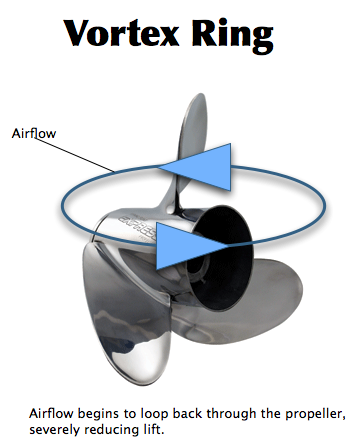
\includegraphics[width=85mm]{imageSources/vortexRing.png}
  \end{center}
  \captionof{figure}{Vortex Ring Effect} 
  \label{vortexRing}
  \end{minipage}

\subsection{Design Schematics}

The following figures show the top, side, front and rear views for the vehicle:

\begin{minipage}{6.5in}
  \begin{center}
    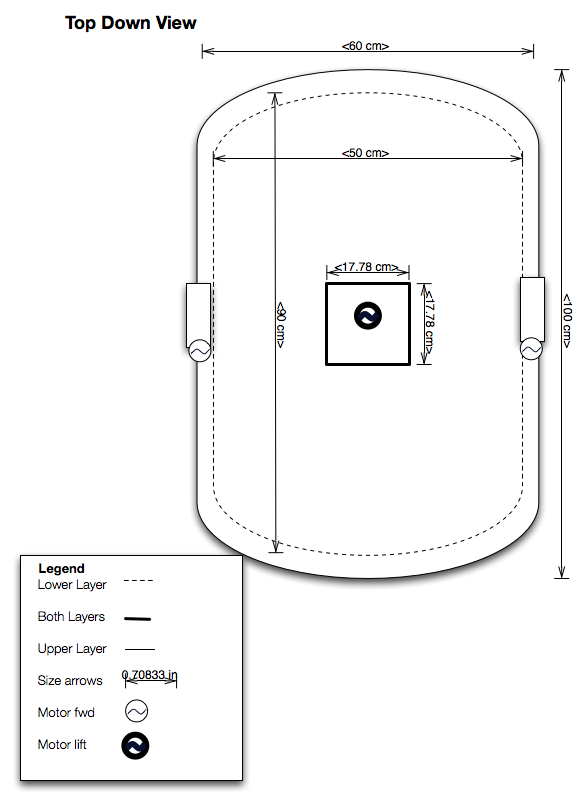
\includegraphics[width=85mm]{imageSources/topDownView.png}
  \end{center}
  \captionof{figure}{Hovercraft: Top Down View} 
  \label{topDownView}
\end{minipage}

The first design consisted of a rounded front, straight sides and a straight back. However, since the front and back were not symmetric, it was concluded that the rear of the craft should be rounded to match the front. This symmetric design better distributed the underlying air cushion to all parts of the vehicle.

  \begin{minipage}{6.5in}
  \begin{center}
    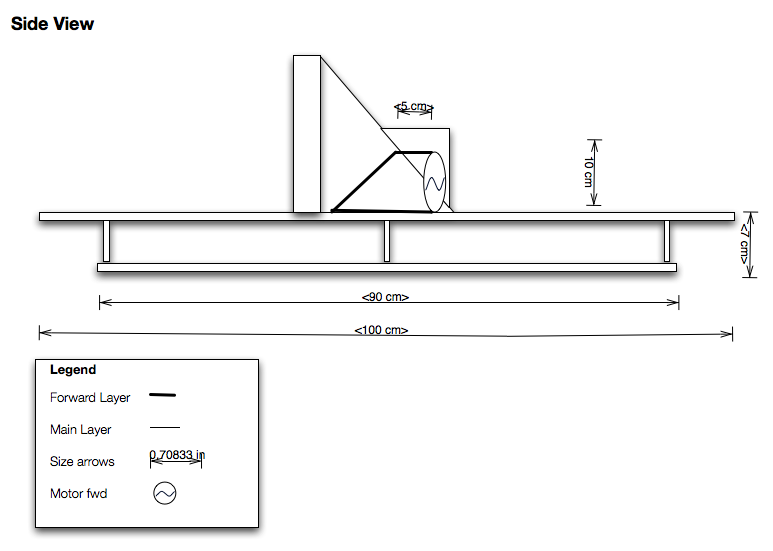
\includegraphics[width=85mm]{imageSources/sideView.png}
  \end{center}
  \captionof{figure}{Hovercraft: Side View} 
  \label{sideView}
  \end{minipage}

The plenum chamber receives air from a single propeller mounted in the middle of the chassis. The middle propeller is housed by a triangular container. Initially the container was completely open on the side where the propeller draws air from. Too much air was escaping from this hole and a cover with a circular cut-out was fitted over the opening. The cut-out better fit the diameter of the fan, resulting in minimal air escaping from the opening.

  \begin{minipage}{6.5in}
  \begin{center}
    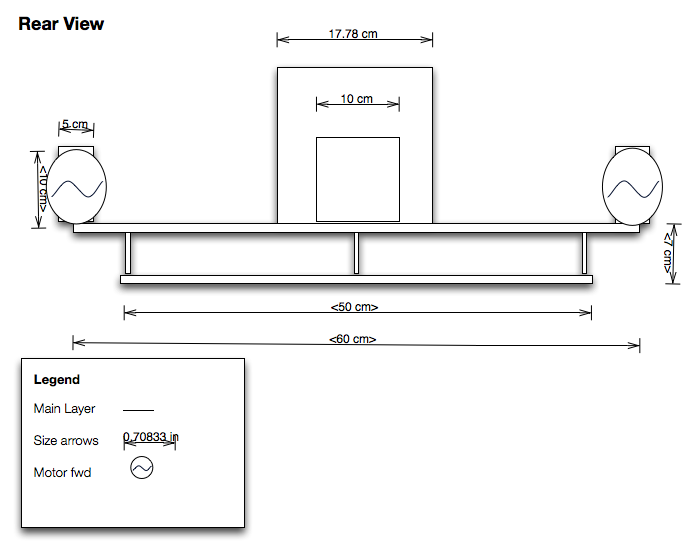
\includegraphics[width=85mm]{imageSources/rearView.png}
  \end{center}
  \captionof{figure}{Hovercraft: Rear View} 
  \label{rearView}
  \end{minipage}

The electronic components were mounted at the rear of the hovercraft. This facilitated making connections from the breadboard to the nearby DC Motors, servo motor, and sonars. The combined mass of all the components added a significant force to the rear of the chassis. To counter this, counter weights were placed on the front of the body.

\begin{minipage}{6.5in}
  \begin{center}
    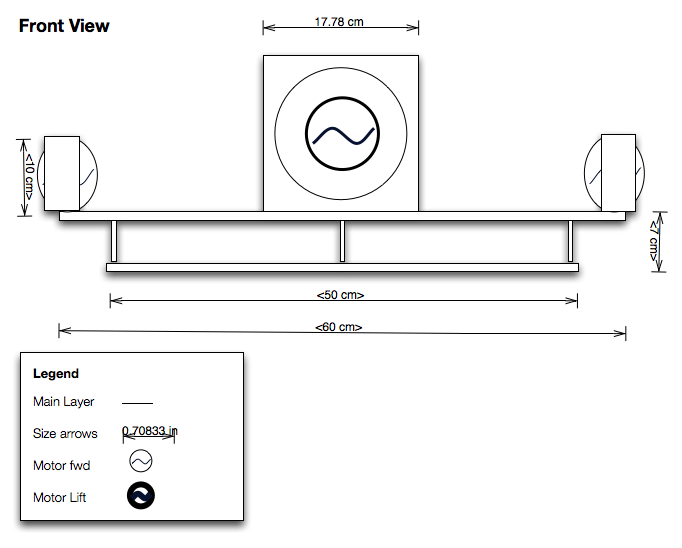
\includegraphics[width=85mm]{imageSources/frontView.png}
  \end{center}
  \captionof{figure}{Hovercraft: Front View} 
  \label{frontView}
\end{minipage}

\subsection{Design Constraints}
The following constraints were issues that needed to be met by the resulting hovercraft design.

\subsubsection{Payload Weight}
In order for the hovercraft to stay afloat, the internal air pressure must counter external forces placed on the surface of the vehicle by both gravity and the mass of the components. The following table describes the components and their masses:

\begin{minipage}{6.5in}
\captionof{table}{Weight of Hovercraft Components}
\begin{center}
\begin{tabular}{ c c c}
  Component & Quantity & Weight (grams) \\
  \hline
	Battery  &	2 & 	50 \\
	Breadboard &	1 &	45 \\
	Microcontroller &	1 &	15 \\
	Radio &	1 &	9 \\
	Sonar &	3 &	5 \\
	DC Motor (large) &	1 &	83 \\
	Servo Motor &	1 &	4 \\
	H-bridge &	1 &	6 \\
	DC Motor (small) &	2 &	25 \\
	Total &	-- &	329 \\
\end{tabular}
\end{center}
\label{restingTable}
\end{minipage}

\subsection{Rigidity}
The hovercraft body was made from two thin sheets of styrofoam separated by 12 styrofoam spacers 1'' thick. This proved to be a very strong design, easily capable of supporting the payload of the electronics. In fact, additional weight was distributed evenly across the body and it was found that the hovercraft could support at least 1 kg.

\begin{minipage}{6.5in}
  \begin{center}
    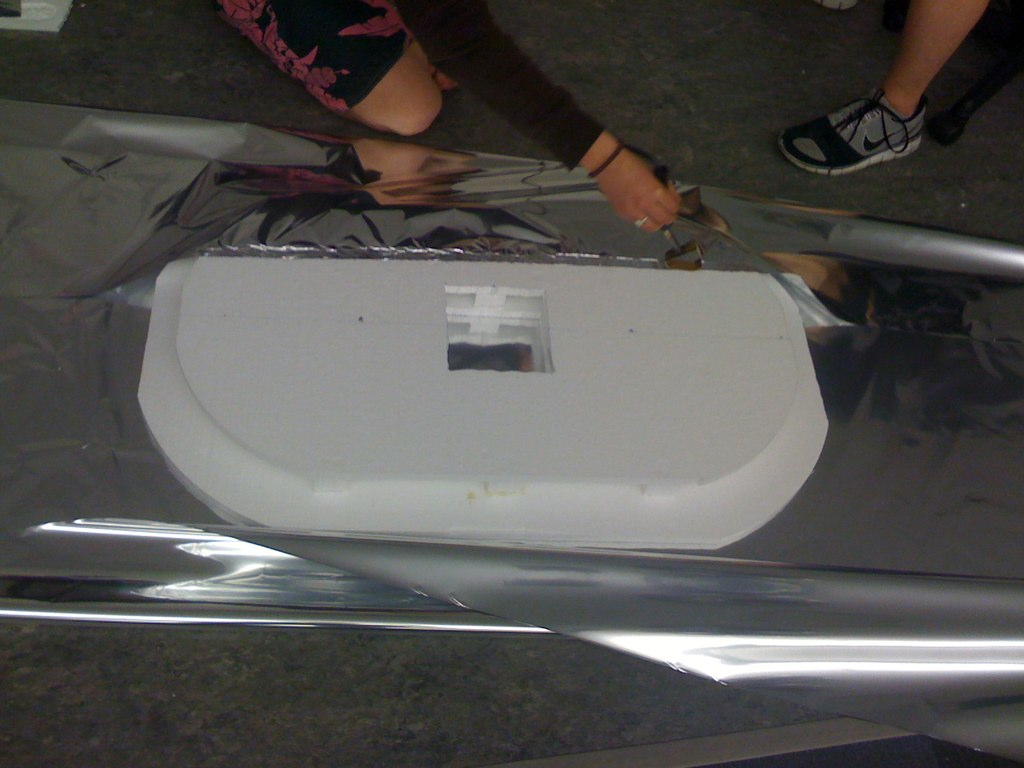
\includegraphics[width=85mm]{imageSources/rigidity1.png}
  \end{center}
  \captionof{figure}{Rigidity of Hovercraft I} 
  \label{rigidity1}
\end{minipage}

\begin{minipage}{6.5in}
  \begin{center}
    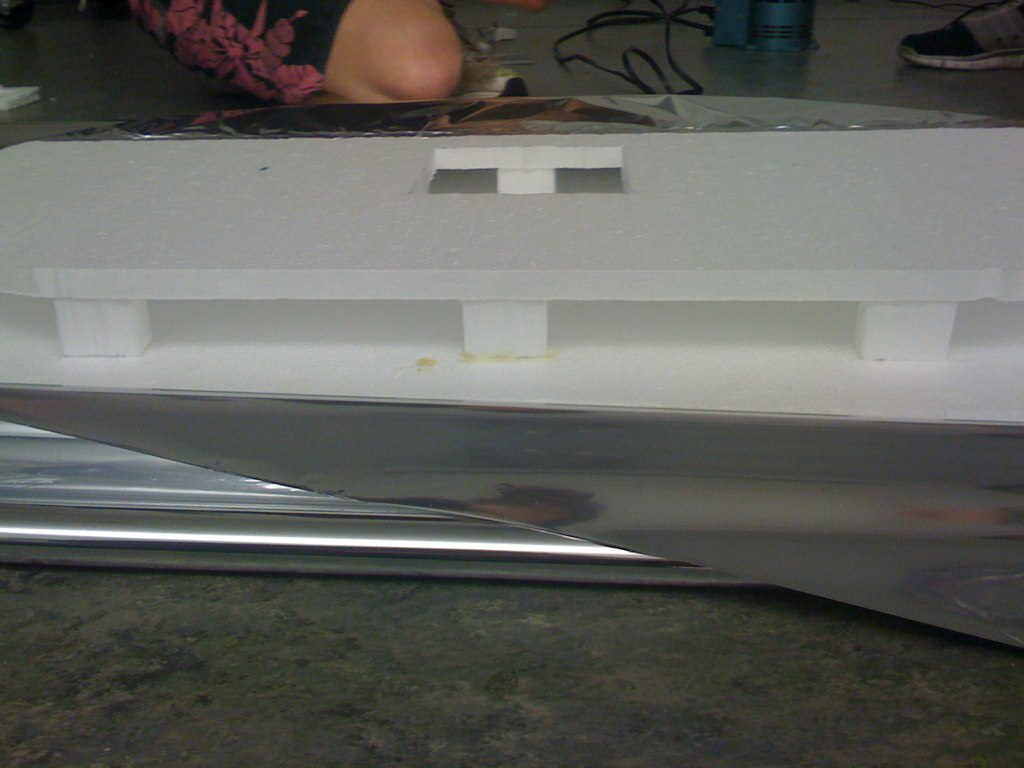
\includegraphics[width=85mm]{imageSources/rigidity2.png}
  \end{center}
  \captionof{figure}{Rigidity of Hovercraft II} 
  \label{rigidity2}
\end{minipage}

An inflatable skirt made of mylar surrounded the body. Mylar is a polyester film often used in flexible packaging for food, as an insulating material, and for solar reflection. Once inflated, the skirt served two purposes. First, because it expanded to over two inches, it provided additional surface area, reducing the overall pressure at any given point on the body. Second, the skirt acted as a flexible and damage resistant bumper, protecting the body from nearby objects during testing. Two different mediums were used to connect the skirt to the styrofoam body. First mylar was adhered to the styrofoam using hot glue.  Next a hot iron was pressed around the perimeter to melt the mylar, the glue and the styrofoam together.

\begin{minipage}{6.5in}
  \begin{center}
    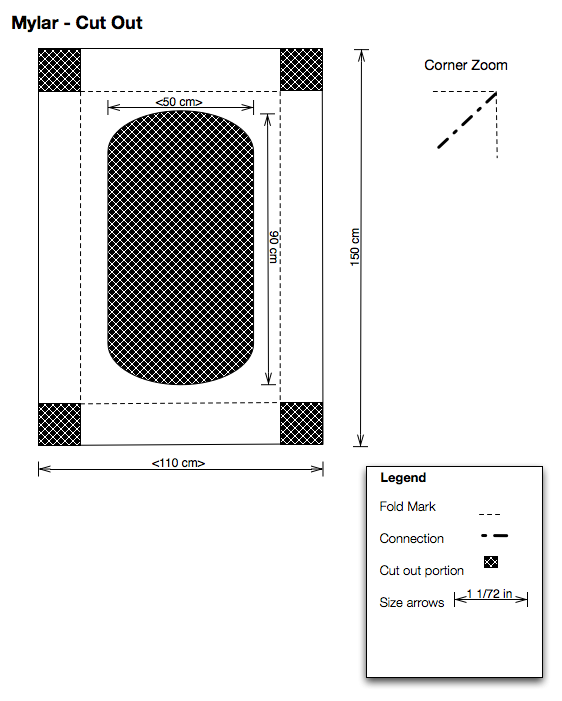
\includegraphics[width=85mm]{imageSources/mylarSchematic.png}
  \end{center}
  \captionof{figure}{Schematic of the Mylar skirt} 
  \label{mylarSchematic}
\end{minipage}

After the styrofoam chassis was built, the skirt of the hovercraft was constructed. The first attempt at constructing the mylar skirt was not successful. Lack of foresight resulted in a skirt that was too baggy in some areas, while exposing too many holes in others. The first time the mylar was attached, each of the corners was connected using clear packing tape, simply folding the corners together. The second attempt was much more calculated and pragmatic. When connecting the corners of the second skirt, the edges were methodically folded in, and the resulting square that was not attached was removed (see Figure mylarSchematic). Connections were then made using the hot iron to glue the seam together. The resulting skirt was much more evenly distributed and provided reasonably uniform inflation around the entire body. That said, the hovercraft still managed to move about when it was supposed to be idle. An attempt to address this issue was made by placing weights on the body to counteract the uneven escape of air on one side.

\subsubsection{Lift}
The decision to use a single, vertically mounted propeller to feed air into the plenum chamber was in direct response to the problem of rotational torque plaguing horizontally mounted propellers. In a horizontal design, the rotation of the blades applies an overall torque on the hovercraft causing it to spin. Dealing with this force is a burden. One approach is to install a second horizontal propeller which spins in the opposite direction. The opposite spin of the two motors cancels any directional torque felt by the craft. The problem was avoided entirely by mounting a single motor vertically in the middle of the body. A container built over the propeller captured the incoming air and forced it into the plenum chamber.

\begin{minipage}{6.5in}
  \begin{center}
    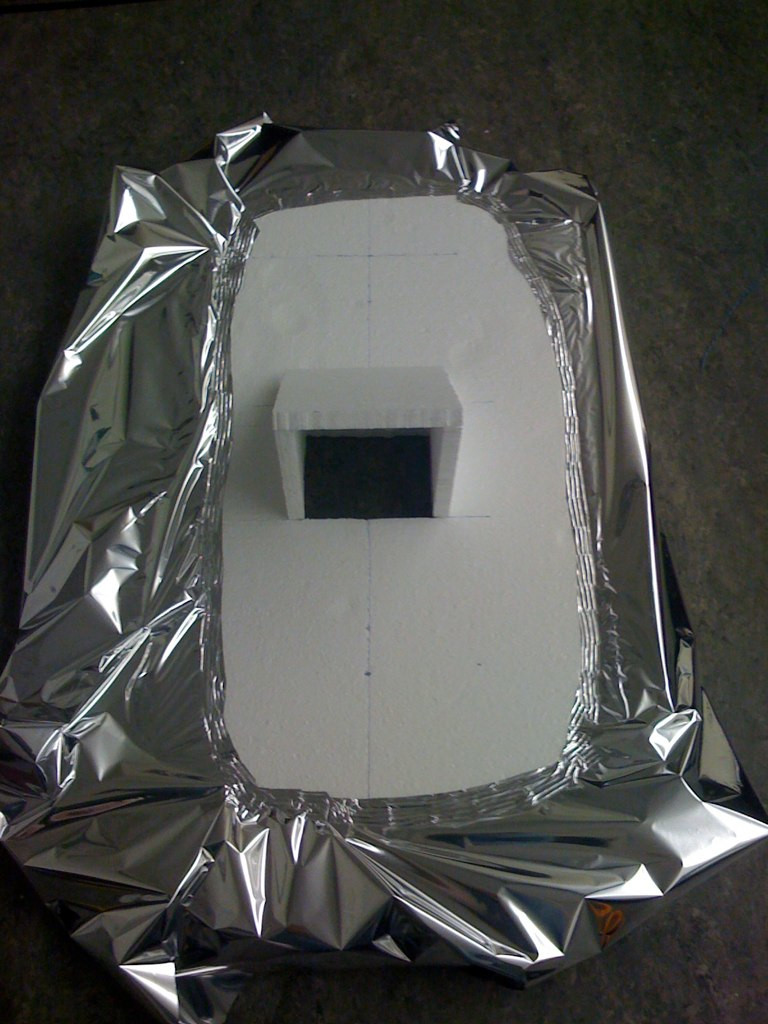
\includegraphics[width=85mm]{imageSources/lift1.png}
  \end{center}
  \captionof{figure}{Hovercraft Lift I} 
  \label{lif1}
\end{minipage}

\begin{minipage}{6.5in}
  \begin{center}
    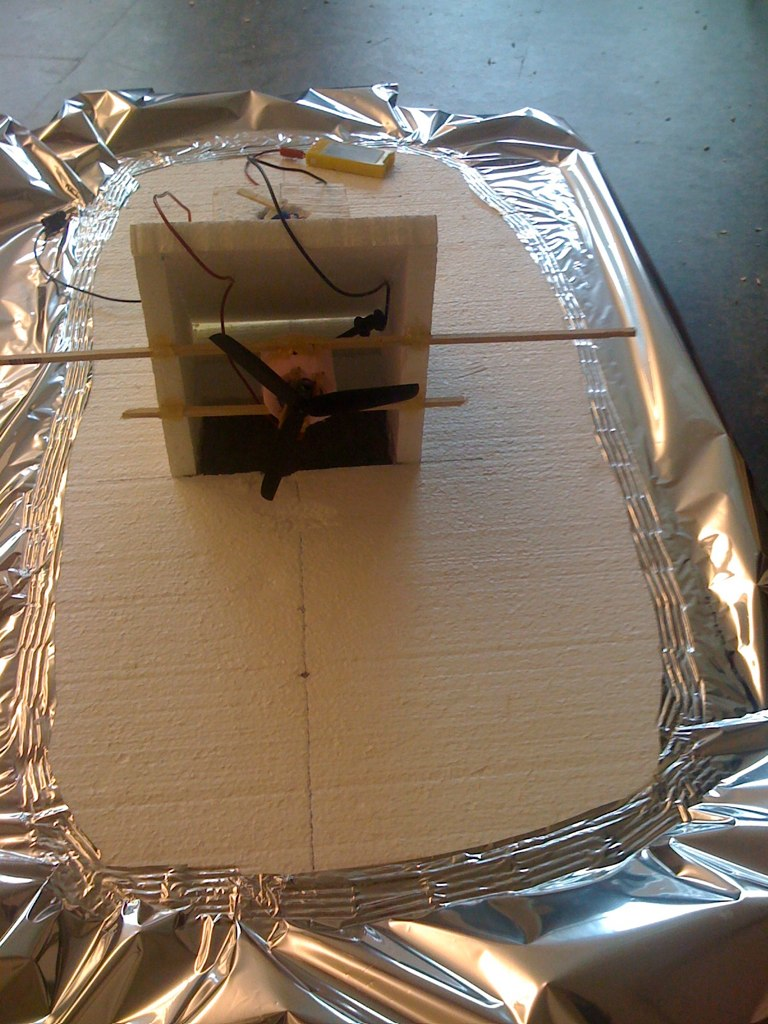
\includegraphics[width=85mm]{imageSources/lift2.png}
  \end{center}
  \captionof{figure}{Hovercraft Lift II} 
  \label{lift2}
\end{minipage}

To avoid ground effect, full power was applied to the lift propeller. Next, weight was incrementally added to the body such that the hovercraft moved freely along the ground, but was not vastly overpowered by the fan. Keeping the vehicle as close as possible to the ground allowed for the most control over the hovercraft's direction.

\subsubsection{Thrust and Control}

Figures \ref{thrustControl1} and \ref{thrustControl2} show the first chosen design to provide the vehicle with thrust. The two differential motors were mounted at the rear, and were spaced fairly close together.

\begin{minipage}{6.5in}
  \begin{center}
    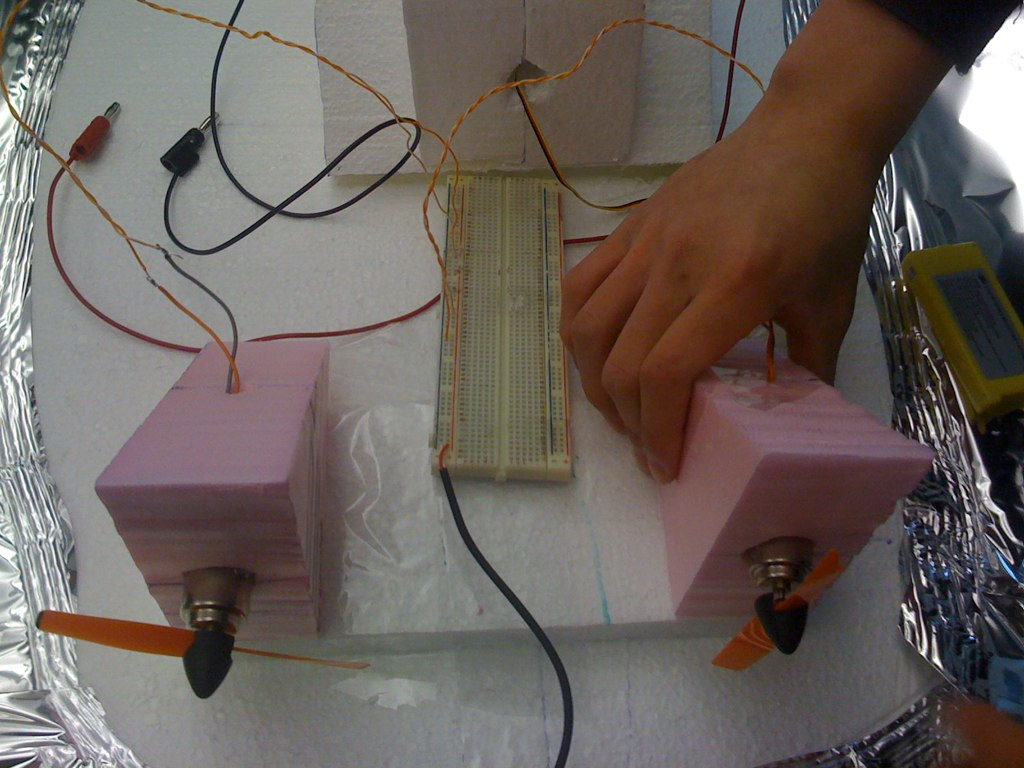
\includegraphics[width=85mm]{imageSources/thrustControl1.png}
  \end{center}
  \captionof{figure}{Hovercraft Thrust and Control I} 
  \label{thrustControl1}
\end{minipage}

\begin{minipage}{6.5in}
  \begin{center}
    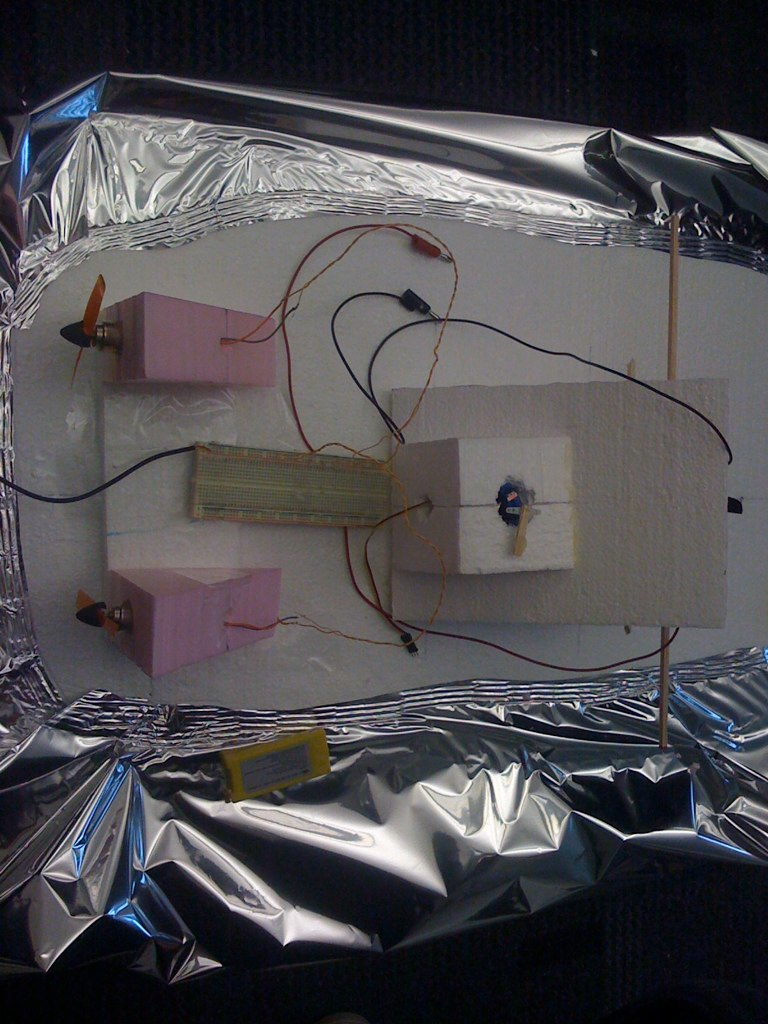
\includegraphics[width=85mm]{imageSources/thrustControl2.png}
  \end{center}
  \captionof{figure}{Hovercraft Thrust and Control II} 
  \label{thrustControl2}
\end{minipage}

This design, however, was soon altered. By placing the motors as far apart as possible, maximum torque could be achieved. The analogy is as follows. Consider the act of opening a door. It is much easier to open a door if one pushes on the edge furthest from the hinges, because more torque can be generated. The same principle applies to the hovercraft. Ideally the centre of rotation (the hinge) is in the centre of the hovercraft. The motors were placed at extreme distances from center (on either side), resulting in maximal rotational torque.   The increased torque allowed for superior control over the vehicle \cite{831309}. 

\subsection{Design Problems and Future Considerations}
The following subsections describe the most challenging problems encountered as the hovercrafts took shape.  

\subsubsection{Shape}
The hovercraft is oval-shaped with a length to width ratio of 3:2. The first problem encountered with this shape was that it was hard to evenly wrap the mylar around the soft corners. The mylar creased around the corners, and stuck out unevenly, often hanging down enough to provide friction for the hovercraft, creating a pivot point when the hovercraft tried to move around around.  Extra cuts were needed, as well as ironing and gluing the corners.  A hovercraft with sharper edges may take significantly less mylar tuning, and speed has not been found to be a major issue, so the fact that square edges may reduce the aerodynamics of the hovercraft may not be as significant an issue as previously thought.

\subsubsection{Weight Distribution}
The air intake fan forced air parallel to the ground, and a Styrofoam encasing around the fan directed the air down into the hovercraft base, with a single hole at the bottom of the hovercraft in the center. As mentioned above, the mylar was sealed around the edges of the hovercraft so that it was air-tight. A Styrofoam circle was cut having a diameter just slightly bigger than that of the fan; it was placed even with the edge of the fan in order to get the maximum possible amount of air intake and prevent as little air as possible from escaping.  The fan motor was large, and was able to easily lift the hovercraft.  This design hasn't suffered from any lift-related issues. The main problem encountered by using a single large fan was that it was being held up by the small square Styrofoam encasing, under 20cm in length. The fan made up a significant portion of the overall weight of our hovercraft, and the weight distribution is all in the very center of the hovercraft. Because a large amount of the weight was in the very center, the hovercraft can easily tip, allowing air to flow out from the bottom of one side, resulting in the hovercraft gliding across the floor, or spinning.

\begin{minipage}{6.5in}
\begin{center}
  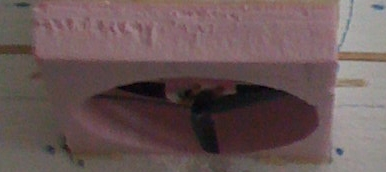
\includegraphics[width=85mm]{imageSources/weightDistro1.png}
\end{center}
\captionof{figure}{Weight Distribution I} 
\label{weightDistro1}
\end{minipage}

\begin{minipage}{6.5in}
\centering
  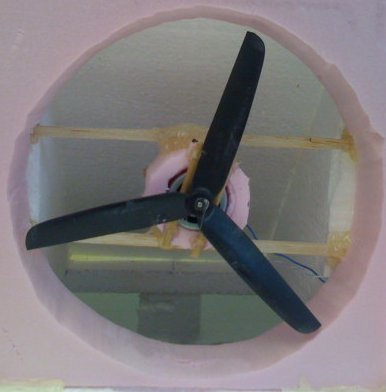
\includegraphics[width=85mm]{imageSources/weightDistro2.png}

\captionof{figure}{Weight Distribution II} 
\label{weightDistro2}
\end{minipage}

If the hovercraft moved around at all when just the lift fan was on, it became extremely hard to control with the joystick. It was hoped that such a problem could be counterbalanced with software, and shift the power of the thrust motors on the side of the hovercraft accordingly. This took a lot of fine-tuning, and the hovercraft still was extremely hard to control, as air always seemed to be leaking from a different side, depending on the hovercraft's current movement direction and the forces exerted by the fans.

By placing weight around the edges of the hovercraft, the movement of the hovercraft was greatly reduced when just the lift fan was on. The problem was that when enough weight was placed around the perimeter of the hovercraft that it remained motionless when the thrust motors were off, the fans had trouble moving the hovercraft forward or backward even at full power. As weight was removed, the motors could control the hovercraft more, but with less weight balancing the hovercraft, it again moved and spun uncontrollably.

\subsubsection{Turning Pivot}
The motors were originally placed at the back end of the hovercraft, as shown in the Figure \ref{turningPivot1}.  It was determined that the turning pivot of the hovercraft was directly in-between where the two thrust motors were placed. With the turning pivot at the back end of the hovercraft, the turning radius of the center of the hovercraft was equal to about half of the hovercraft's length (~90cm), and it was difficult and awkward to control the hovercraft correctly. 

\begin{minipage}{6.5in}
\begin{center}
  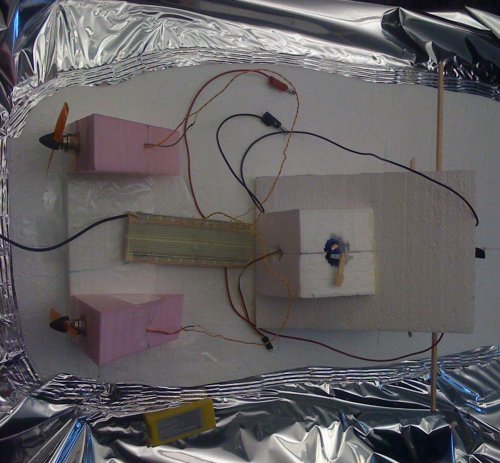
\includegraphics[width=85mm]{imageSources/turningPivot1.png}
\end{center}
\captionof{figure}{Turning Pivot I} 
\label{turningPivot1}
\end{minipage}

The thrust motors were shifted so that the fan blades were at the very center of the hovercraft. This allowed the hovercraft to have much tighter turns, and reduced its turning radius so that the its pivot was right at the center. Controlling the hovercraft was much more intuitive this way.

\begin{minipage}{6.5in}
\begin{center}
  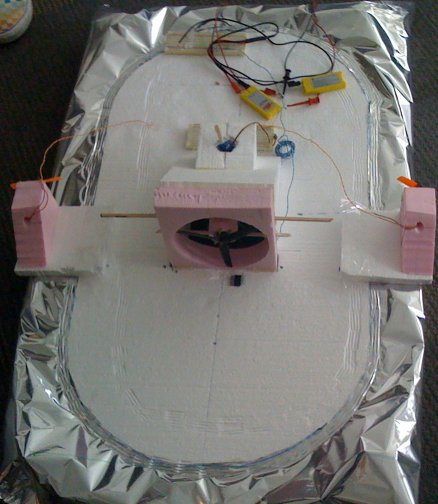
\includegraphics[width=85mm]{imageSources/turningPivot2.png}
\end{center}
\captionof{figure}{Turning Pivot II} 
\label{turningPivot2}
\end{minipage}

\subsubsection{H-bridge}
One of the challenges encountered was that thrust motors were not receiving enough power. This lack of thrust made it nearly impossible to accelerate in either direction. In the initial testing, thrusting motors were connected directly to the 7 volt power source. In this experiment, the craft moved forward at a very quick speed over both the smooth linoleum floor and the carpet.

When testing the H-Bridge independently, it seemed like there was sufficient power being supplied to the thrust motors. Once the H-bridge and motors were connected through the bread-board, along with the radio, and other components, the hovercraft hardly moved. The fans were moving much too slowly to accelerate the vehicle. The initial hypothesis was that there was not enough voltage being supplied to the H-Bridge. To solve this problem, an extra battery was connected to one side of the bread-board to power the H-Bridge side, and another to control the other components on the bread-board. This solution did not seem to affect the thrust motors' power at all, as they still did not spin fast enough to accelerate the hovercraft.

Reading the documentation about the L293D H-Bridge revealed that it can only handle 1.5A maximum. At this point a higher amperage H-Bridge was substituted in. Again, the H-Bridge was wired up independently, the motors spun very well, and significantly faster than with the previous L293D H-Bridge. Unfortunately, when it was tested with the rest of the components, the motors seemed to jitter, sometimes spinning as powerfully as needed, but very irregularly. It was thought this irregularity was due to a faulty H-Bridge, so the smaller L293D H-Bridges was replaced because it was known that this component functioned correctly. As the 1.5A maximum was the limiting factor with the L293d H-Bridges, it was decided that the wiring should be done in parallel. At 5 volts, this solution gave the fans almost enough power to control the hovercraft sufficiently. Unfortunately, when 7 volts were applied, again the power shifted irregularly. Another problem was that over 30 of the bread-board's 67 pins were being used for the H-Bridges and Inverters alone, not leaving enough room for the other necessary components. It was later discovered that the H-bridges could be `piggy-backed' by soldering them on top of one another. This would solve the lack of pins issue. It has also since been discovered that the irregular power issues were caused by the H-Bridges becoming too hot and shutting off. Attaching a heat-sink solved this problem, which is discussed below, so two L293D H-Bridges may be a very viable option!

\begin{minipage}{6.5in}
\begin{center}
  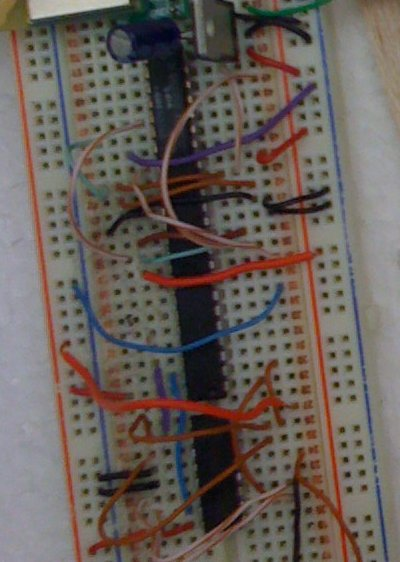
\includegraphics[width=85mm]{imageSources/designProblemsHBridge1.png}
\end{center}
\captionof{figure}{H-bridge Wiring Alternative I} 
\label{HbridgeWiring}
\end{minipage}

\begin{minipage}{6.5in}
\begin{center}
  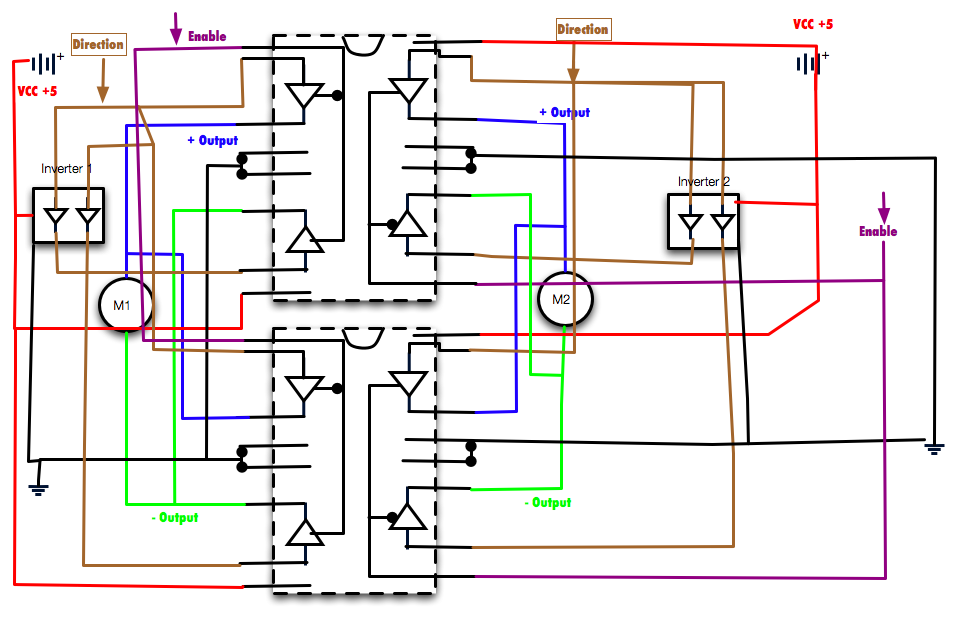
\includegraphics[width=85mm]{imageSources/designProblemsHBridge2.png}
\end{center}
\captionof{figure}{H-bridge Wiring Alternative II} 
\label{HbridgeWiring2}
\end{minipage}

At this point, another high-amperage H-Bridge was acquired. The new H-Bridge also had an attached heat-sink. This heat-sink would prevent the H-Bridge from becoming too hot and temporarily shutting off. With the heat-sink, the motors were getting enough power to successfully control the hovercraft, and the heat-sink prevented the irregular shifts in power caused by the H-Bridge shutting off.

\begin{minipage}{6.5in}
\begin{center}
  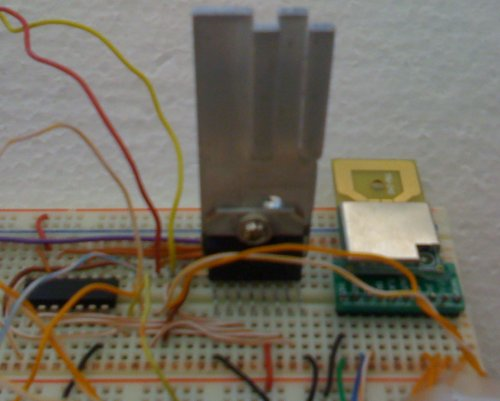
\includegraphics[width=85mm]{imageSources/designProblemsHBridgeHeatsink.png}
\end{center}
\captionof{figure}{H-bridge Heatsink} 
\label{HBridgeHeatsink}
\end{minipage}

\subsubsection{Joystick}
\label{sec:JoystickConst}
The joystick provided seemed to be very unstable, producing inconsistent values and refusing to maintain its center position. This made it very difficult to write suitable software to produce consistent results. Eventually a new joystick was acquired that had not yet been modified to connect and work with the AT90. The joystick was dismantled, revealing that it was currently using three potentiometers. One of the potentiometers was for the X position of the joystick, another was for the Y position, and the third was for the position of a dial on the base of the joystick. These potentiometers were connected so that the amount of current was determined by the position of the joystick, or the dial.

A potentiometer is a resistor with three terminals: a ground, an input, and an output (the wiper). There is a knob connected that can be spun, and as the knob is turned, the middle pin reads the voltage, and will output a reading that is the difference between ground, (zero) and the value of the input (in our case VCC).

\begin{minipage}{6.5in}
\begin{center}
  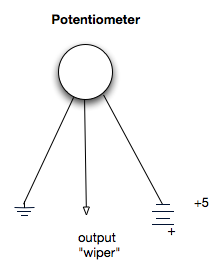
\includegraphics[width=85mm]{imageSources/joystickPotentiometer.png}
\end{center}
\captionof{figure}{Joystick Potentiometer} 
\label{joystickPotentiometer}
\end{minipage}

The potentiometer at the base of the joystick was removed, allowing the hovercraft to be controlled more simply with only X- and Y-coordinates. The two remaining potentiometers were modified and connected so that the amount of voltage was determined by the position of the joystick. To do this one side of the potentiometer was grounded, and connected power to the other. The middle connection was then connected through the serial port as output. The current implementation outputs all three values at the base station, and sends them to the hovercraft. Future implementations may end up using the dial at the base of the joystick to control a ``side-stepping'' fan connected to the hovercraft that blows air perpendicular to the other fans. This would prevent the hovercraft from having to zig-zag down a hallway, as this fan could blow air toward the close wall to ``side-step'' the hovercraft away from the wall, without having to make an actual turn.

\begin{minipage}{6.5in}
\begin{center}
  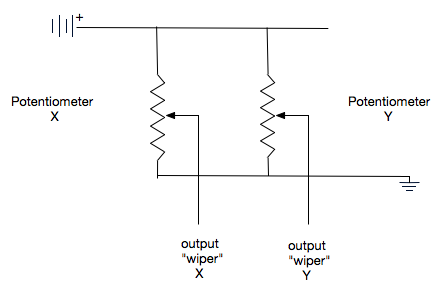
\includegraphics[width=85mm]{imageSources/potentiometerSchematic.png}
\end{center}
\captionof{figure}{Joystick Potentiometer Schematic} 
\label{potentiometerSchematic}
\end{minipage}

Once the casing was replaced on the joystick, the readings from the board, when the joystick was connected to 5 volts of regulated power, are displayed in the table below.

\begin{minipage}{6.5in}
\captionof{table}{Joystick Voltage for Direction}
\begin{center}
\begin{tabular}{ c c }
  Position & Reading (volts) \\
  \hline
  Forward & 3.76 \\
  Middle & 2.278 \\
  Backward & 0.633 \\
\end{tabular}
\end{center}
\label{voltagePotentiometerTable}
\end{minipage}

\subsection{The Second Hovercraft}
Several different designs were attempted when trying to create the second hovercraft. Although the original length to width ratio
of 3:2 was maintained, the second hovercraft was quite a lot smaller, at 45.7cm (18 inches) in length, and 38.1cm (15 inches) in width.
After measuring, cutting, and gluing the Styrofoam, a hovercraft model was created using the Autodesk Maya\footnote{ http://usa.autodesk.com/adsk/servlet/index?siteID=123112\&id=7635018 }
program, and used the program to model a skirt onto the hovercraft.

\begin{minipage}{6.5in}
\begin{center}
  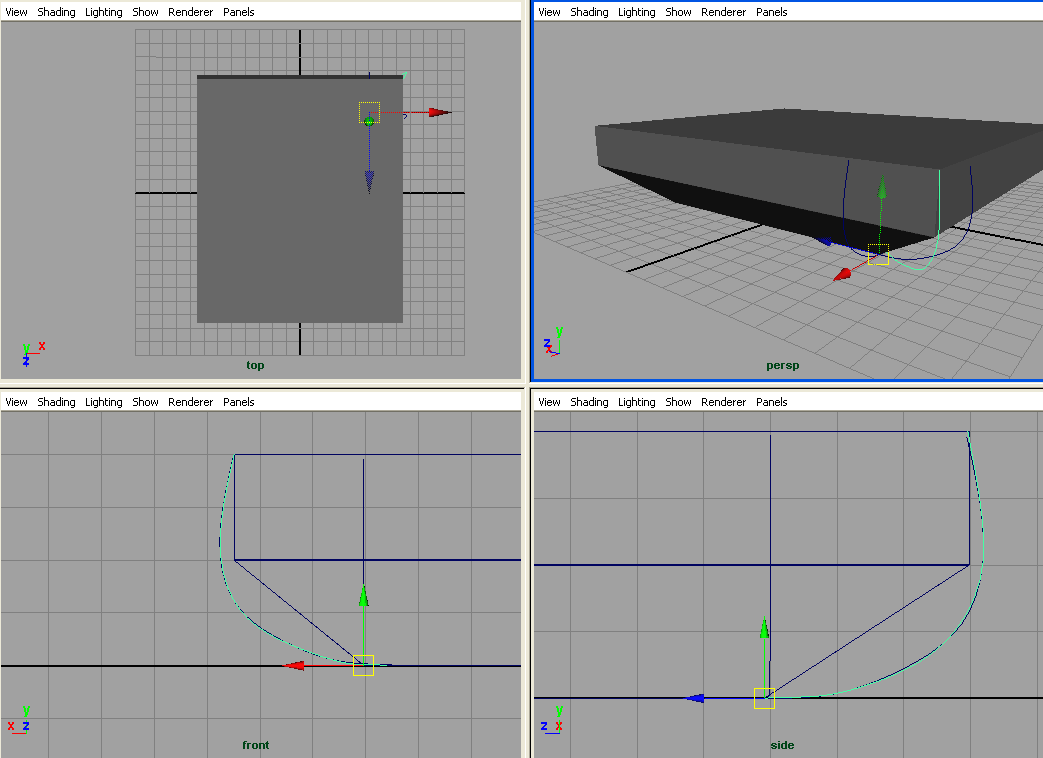
\includegraphics[width=85mm]{imageSources/maya.png}
\end{center}
\captionof{figure}{Using the maya software to view the hovercraft from multiple angles to create the right mylar curve}
\label{maya}
\end{minipage}

As one can see in Figure \ref{maya}, a virtual model of the hovercraft was created 18 units by 15 units, corresponding
to the dimensions of the Styrofoam hovercraft in inches.  A curve was created between the two places on the hovercraft where the skirt would eventually be added.
The curve was manipulated until it was possible to place the same shaped curve around both the lengths and widths of the hovercraft
so they met up perfectly along the corners. It was then possible to flatten the plane to get the desired shape of the mylar piece 
to cut. The image was scaled and printed so it could be traced from the sheet of mylar. This helped avoid the mylar
problem associated with the first hovercraft, where it bunched up and creased around the corners. After cutting the shapes the correct sizes,  many very small pieces of tape were used to tape the 4 pieces of mylar skirt together down the curved corners.  The skirt was then turned inside out (so the tape was on the inside,
and so would not peel off).  A glue gun was used to seal the edge around the outside.  The following subsections will give
brief descriptions of the lift and thrust motor designs that were created and tested, the reasoning behind several design decisions, and the positive and negative results found during testing.

\subsubsection{The First Prototype - Dual side air intake lift fans}

\begin{minipage}{6.5in}
\begin{center}
  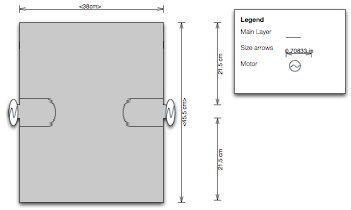
\includegraphics[width=85mm]{imageSources/top2.png}
\end{center}
\captionof{figure}{A top view of the dual side fan prototype} 
\label{top2}
\end{minipage}

A major design goal of the second vehicle was the weight distribution of the center fan, and the reduction of the fan motor size required to lift the hovercraft. In the first
prototype, two fans were used to lift the hovercraft, placed half-way between the front end
and back end of the vehicle. Instead of having the fans blow air down towards the ground, the fans were placed at each side
of the hovercraft; they forced air parallel to the ground, into the hovercraft. As the top of the hovercraft was
air-tight styrofoam, no air escaped from the top.  Mylar was used to make an air-tight skirt again, with two holes cut out
of the bottom of the of both the mylar and bottom layer of styrofoam to let air escape. The hovercraft's length was 18 inches,
and it's width was 15 inches, and the mylar skirt came in 3 inches at the front and back, and 2.5 inches at the left and right,
providing for one third of the total surface area at the bottom of the hovercraft.

\begin{minipage}{6.5in}
\begin{center}
  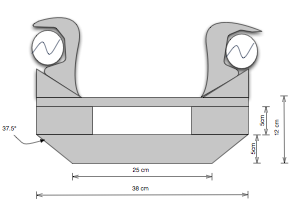
\includegraphics[width=85mm]{imageSources/Front2.png}
\end{center}
\captionof{figure}{A front view showing the two thrust fans} 
\label{Front2}
\end{minipage}

Two thrust fans were mounted directly above the lift fans, at the center of the hovercraft. The thrust motors in the previous
hovercraft were positioned in the same way, and it was felt that with the decreased size and weight of the new prototype, the 
two thrust fans would be able to sufficiently move and steer the hovercraft.

With this design, the hovercraft actually hovered very well: without the thrust fans on, it didn't spin, or move in 
any direction, it simply hovered in place. This was something not achievable with the previous hovercraft design 
without adding a lot of weight and spending a lot of time weight balancing.

\begin{minipage}{6.5in}
\begin{center}
  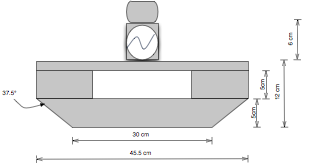
\includegraphics[width=85mm]{imageSources/SideView2.png}
\end{center}
\captionof{figure}{A side view showing one of the air intake fans} 
\label{Side2}
\end{minipage}

When all of the other necessary components were placed onto the hovercraft, the lift was noticeably weaker, and the fans
even sounded as if they were generating a lot less power. By placing a hand in front of either of the lift fans, one could feel
a bit of air coming back out. As weight was added to the hovercraft, there was less space for the air to flow out the bottom
of the hovercraft, and so there was more reverse pressure on the two side fans. For this prototype the smaller fans were used
and they could not sufficiently overpower the back pressure. With both fans at full power, the hovercraft was just barely able
to lift off the ground, and was not even able to hover over very small objects, like the bump separating the Linoleum floor
from the carpeted floor in the lab. 

\subsubsection{The Second Prototype - Single rear lift and thrust motors}

\begin{minipage}{6.5in}
\begin{center}
  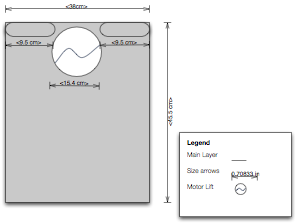
\includegraphics[width=85mm]{imageSources/Topfinal.png}
\end{center}
\captionof{figure}{A top view of the single rear lift  motor prototype} 
\label{finaltop}
\end{minipage}

Because the two smaller fans didn't seem to provide enough power to sufficiently lift the hovercraft with all of the components
attached, the previous design was reexamined, which was to use a single powerful motor to provide the lift for the hovercraft. 

\begin{minipage}{6.5in}
\begin{center}
  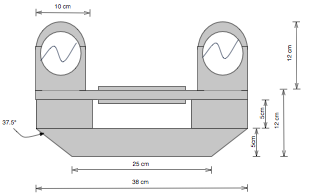
\includegraphics[width=85mm]{imageSources/Frontfinal.png}
\end{center}
\captionof{figure}{A front view showing the two thrust motors, and the lift motor encasing} 
\label{finaltop}
\end{minipage}

In the first hovercraft, the main fan was installed in the center of the chassis.  The other components were placed all around it to 
balance the hovercraft. That strategy ended up being very difficult, because in order to spread out the weight distribution so that
both the front and back end were level, the breadboards had to be spread out, resulting in long connecting wires between the spread
out components. The next prototype saw the main lift fan placed as far back on the hovercraft as possible; the intent was to place all of the other components together at the front end, reducing the amount of messy looking wiring. 

\begin{minipage}{6.5in}
\begin{center}
  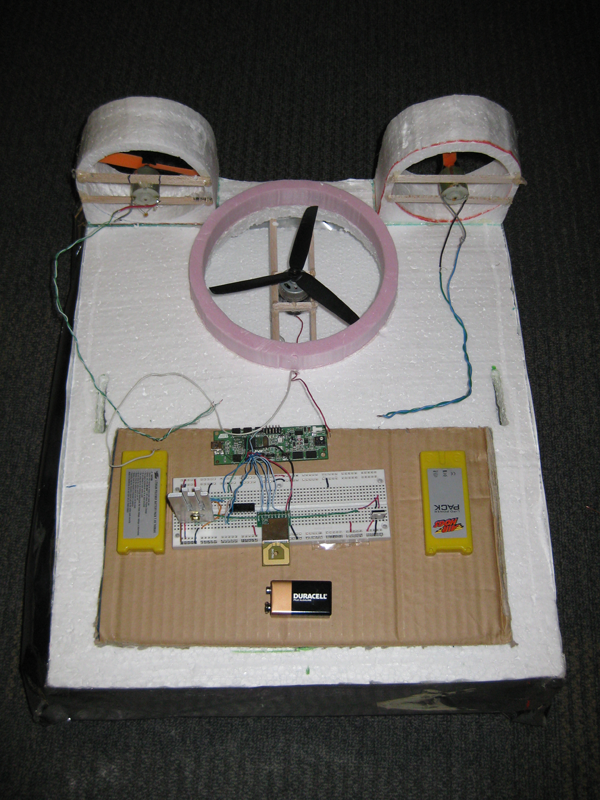
\includegraphics[width=85mm]{imageSources/designProblemsnew_weight.png}
\end{center}
\captionof{figure}{Hovercraft design with fans at the back, and components at the front} 
\label{new_weight}
\end{minipage}

The hovercraft lifted very well with this design, but the lift motor was so strong that it was almost impossible to control
the hovercraft. The skirt was detached from the bottom of the hovercraft, which would provide for more cushioning when
the hovercraft tilted. This provided for even greater lift. The hovercraft lifted over 2 inches off the ground, and it was
possible to slide a textbook right underneath it. The main
problem was that the motors at the back were significantly heavier than the components at the front, so the hovercraft
tilted backwards. When extra weight was added to the front, the hovercraft would still tilt from side to side, resulting
in yet another weight balancing problem.

It was desirable to avoid having to place many different objects around the hovercraft to balance it. This was the approach taken with previous
hovercraft.  Unfortunately it had a serious tilt problem with the back end being so much heavier. A hole was cut in the front center of 
hovercraft to allow air to flow out the front, allowing the hovercraft to level out. This approach worked, but unfortunately
we still faced the tilting problem. Two air slits were inserted down the side of the aircraft to allow a thin stream of air
to flow out each side, and this produced a balanced hovercraft, without having to place weights around the perimeter.
The reasoning behind the air holes was that the hovercraft seemed to always tilt in one direction, because otherwise there
was not enough air escaping. If the hovercraft was pushed down on one side, then the air would flow out the opposite side, and it would have 
an opposite tilt. The air slits down each side helped prevent this phenomenon.

\begin{minipage}{6.5in}
\begin{center}
  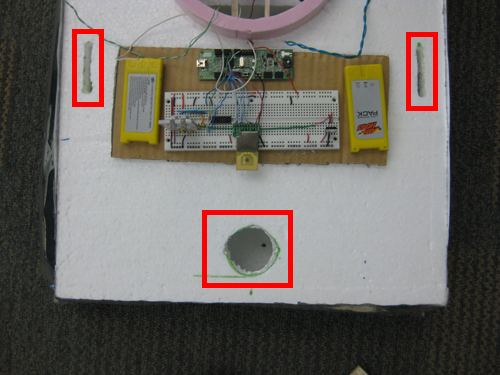
\includegraphics[width=85mm]{imageSources/designProblemsnew_holeshighlighted.png}
\end{center}
\captionof{figure}{Re-balanced hovercraft with air release holes} 
\label{new_holes}
\end{minipage}

As mentioned previously, the skirt was detached from the the bottom of the hovercraft, providing
better cushioning when necessary, which resulted in a greater lift. After making the air holes to balance
the hovercraft, the hovercraft did not lift as far off of the ground as before. Sometimes parts
of the mylar skirt would catch on the floor, slowing or stopping the hovercraft's movement. Half-way down the
sides and length of the skirt it would often droop down to catch on the floor. To fix this problem,
mylar strips were attached across the open space between the sides of the skirt like you can see in Figure \ref{new_bottom}.

\begin{minipage}{6.5in}
\begin{center}
  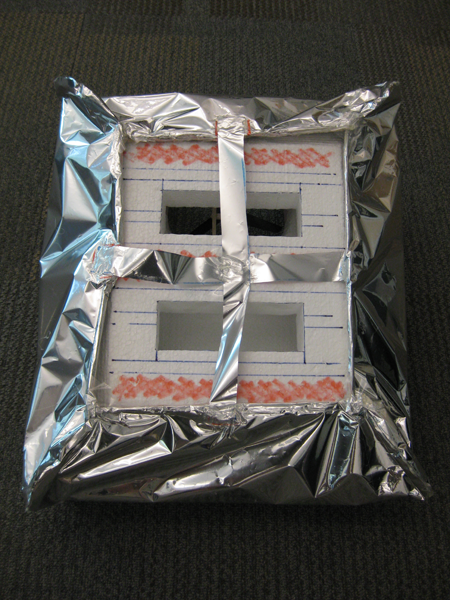
\includegraphics[width=85mm]{imageSources/designProblemsnew_bottom.png}
\end{center}
\captionof{figure}{Attached mylar strips to prevent drooping} 
\label{new_bottom}
\end{minipage}

After attaching the mylar strips, the hovercraft still occasionally got caught up because now the corners 
were drooping and catching on the carpet. The bottom of the mylar was required to be as level as possible, 
and because the mylar is so flimsy, it required support with something rigid. A level bottom of the skirt
was created by gluing balsa wood around the bottom perimeter of the mylar skirt, as show in figure \ref{new_stick}.

\begin{minipage}{6.5in}
\begin{center}
  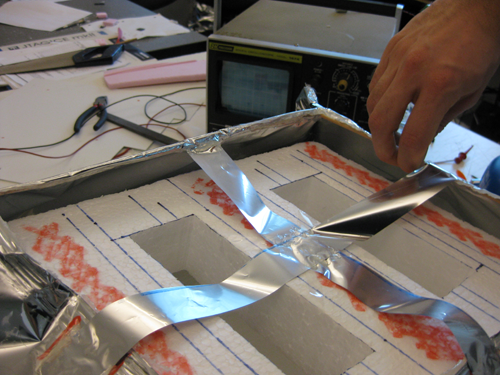
\includegraphics[width=85mm]{imageSources/designProblemsnew_stick.png}
\end{center}
\captionof{figure}{Placing the second piece of balsa wood into the bottom of the mylar skirt} 
\label{new_stick}
\end{minipage}

In the next prototype, the weight distribution of the center fan will be further spread out. This will reduce the amount of weight needed to place around the perimeter to balance the hovercraft, so the motors will be powerful enough to move the hovercraft. Now that the wiring is completed, and the number of batteries, chips, fans, and bread-boards to be used are known.  A new design that takes into consideration their weights as well may be possible. A large lift fan has always easily lifted the hovercraft, but it has been found that have it drains batteries quickly.  The next design will also be a smaller hovercraft size, and therefore will also use a smaller lift fan.

